\section{Methods}

%\subsection{NR simulations}

\begin{frame}{Methods (So Far)}
\begin{columns}

% Left column
\begin{column}{0.5\textwidth}
\begin{tcolorbox}[
    colback=white,
    colframe=blue,
    colbacktitle=blue!50!black!50,
    title=NR simulations,
    fonttitle=\bfseries,
    rounded corners,
    boxrule=1pt,
    left=2mm, right=2mm, top=1mm, bottom=1mm
]
\begin{itemize}   
   \scriptsize
    \item Original THC Simulations full GRhydro + M1 (Radice \& Benuzzi 2023, Benuzzi et al. 2025; Gutierrez et al. 2024)
    \item Athena++ extensions (Stone et al. 2020)
    \begin{itemize}
       \scriptsize
        \item Time-dependent BC in Schwarzschild
        %\item Schwarzschild Metric
        \item $q = w q_{\rm nuclear} + (1-w) q_{Helmholtz}$
        %\begin{itemize}
	%	\scriptsize
	%	\item $w\rightarrow 1$ for large $T,\rho$ 
	%	\item $w\rightarrow 0$ for low   $T,\rho$ 
       %\end{itemize}
       \scriptsize
        \item \sout{Nuclear heating tabulated as Wu et al. 2021}
        \item New fits from Magistrelli 
    \end{itemize}
\end{itemize}
 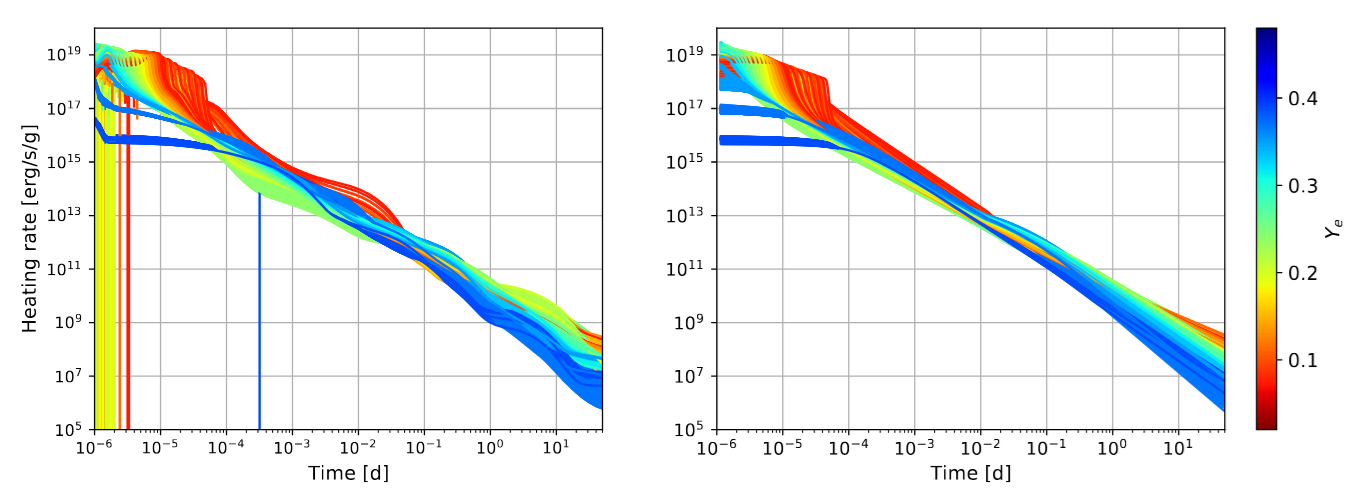
\includegraphics[width=1\linewidth]{../fig/fits.png}
\end{tcolorbox}


\end{column}

% Right column
\begin{column}{0.5\textwidth}
\vspace{-0.5cm}
\begin{tcolorbox}[
    colback=white,
    colframe=blue,
    colbacktitle=blue!50!black!50,
    title=Post-processing,
    fonttitle=\bfseries,
    rounded corners,
    boxrule=1pt,
    left=2mm, right=2mm, top=1mm, bottom=1mm
]
\begin{itemize}
   \scriptsize  
    \item KNEC code for light curves
    \begin{itemize} 
	\scriptsize
	\item 	Magistrelli et al. 2025
    \end{itemize}
   \scriptsize
    \item WinNet for nucleosynthesis
    \begin{itemize}
	\scriptsize
	\item fed with backwards time integrated tracers
	\item enough tracers to resolve the total mass $\sim{4.2}\times10^{4}$
	\item Reichert et al. 2023
    \end{itemize}
\end{itemize}
 
\includegraphics[width=0.6\linewidth]{../fig/winnet_logo_light_theme.png}
\end{tcolorbox}

\end{column}


\end{columns}

\end{frame}

\begin{frame}{Methods (Developments)}
\begin{columns}

% Left column
\begin{column}{0.5\textwidth}
\begin{tcolorbox}[
    colback=white,
    colframe=blue,
    colbacktitle=blue!50!black!50,
    title=NR simulations,
    fonttitle=\bfseries,
    rounded corners,
    boxrule=1pt,
    left=2mm, right=2mm, top=1mm, bottom=1mm
]
\begin{itemize}   
   \scriptsize
    \item Original THC Simulations full GRhydro + M1 (Radice \& Benuzzi 2023, Benuzzi et al. 2025; Gutierrez et al. 2024)
    \item Athena++ extensions (Stone et al. 2020)
    \begin{itemize}
       \scriptsize
        \item Time-dependent BC in Schwarzschild
        %\item Schwarzschild Metric
        \item $q = w q_{\rm nuclear} + (1-w) q_{Helmholtz}$
        %\begin{itemize}
	%	\scriptsize
	%	\item $w\rightarrow 1$ for large $T,\rho$ 
	%	\item $w\rightarrow 0$ for low   $T,\rho$ 
       %\end{itemize}
       \scriptsize
        \item \sout{Nuclear heating tabulated as Wu et al. 2021}
        \item \sout {New fits from Magistrelli}
        \item RHINE
	 \begin{itemize} 
	\item Need of simulations with initial Rhine input data
	\item Not available for THC simulations? Work-around?
	 \end{itemize}
	
    \end{itemize}
\end{itemize}

\end{tcolorbox}


\end{column}

% Right column
\begin{column}{0.5\textwidth}
\vspace{-0.5cm}
\begin{tcolorbox}[
    colback=white,
    colframe=blue,
    colbacktitle=blue!50!black!50,
    title=Rhine,
    fonttitle=\bfseries,
    rounded corners,
    boxrule=1pt,
    left=2mm, right=2mm, top=1mm, bottom=1mm
]

 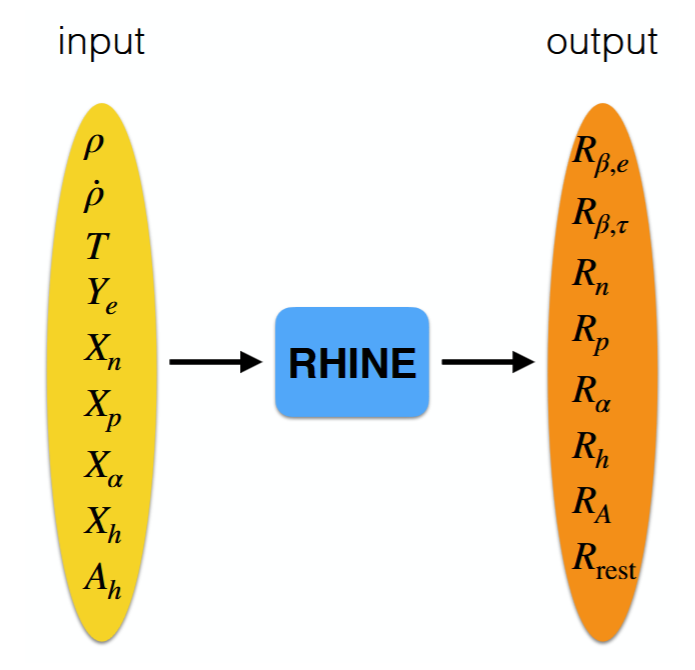
\includegraphics[width=1\linewidth]{../fig/rhine.png}
\end{tcolorbox}

\end{column}

\end{columns}

\end{frame}


\begin{frame}{Methods (Developments - MHD)}
\begin{columns}

% Left column
\begin{column}{0.5\textwidth}
\begin{tcolorbox}[
    colback=white,
    colframe=blue,
    colbacktitle=blue!50!black!50,
    title=GRMHD simulations,
    fonttitle=\bfseries,
    rounded corners,
    boxrule=1pt,
    left=2mm, right=2mm, top=1mm, bottom=1mm
]
\begin{itemize}   
   \scriptsize
    \item Original THC Simulations full GRhydro + M1 (Radice \& Benuzzi 2023, Benuzzi et al. 2025; Gutierrez et al. 2024)
    \begin{itemize}
    	\item Athena++ extensions (Stone et al. 2020)
    	\item Superimpose $\vec{B}$-fields
   \end{itemize}
    \item Original AthenaK Simulations full GRMHD + M1 
    \begin{itemize}
    	\item Athena++ extensions (Stone et al. 2020)
    	\item With $\vec{B}$-fields data
   \end{itemize}

\end{itemize}

\end{tcolorbox}


\end{column}

% Right column
\begin{column}{0.5\textwidth}
\vspace{-0.5cm}
\begin{tcolorbox}[
    colback=white,
    colframe=blue,
    colbacktitle=blue!50!black!50,
    title=$\vec{B}$ injection,
    fonttitle=\bfseries,
    rounded corners,`
    boxrule=1pt,
    left=2mm, right=2mm, top=1mm, bottom=1mm
]

\begin{itemize}
\item What $\vec{B}$ field to superimpose ?
 	\begin{itemize}
	\item $ \vec{B} = \vec{B}_{pol}(1+\psi(r,\theta,\phi,t ,\vec{k})) + \vec{B}_{tor}(\delta(r,t, \vec{l}))$
	\item $\vec{k}$ and $\vec{l}$  are random wave lengths coefficients  
	\item More motivated randomization?
	\end{itemize}
\item Simulated $\vec{B}$-fields ?
 	\begin{itemize}
	\item Wave lengths of $\vec{B}$ may need to match new grid
	\item Cartesian $\rightarrow$ Spherical grids matching
 	\end{itemize}

\end{itemize}   


\end{tcolorbox}

\end{column}

\end{columns}

\end{frame}


\begin{frame}{Models}


\begin{tabular}{c| c| c| c| c| c| c}
\hline\hline
Model & EOS & $M_{1}[M_{\odot}]$ & $M_{2}[M_{\odot}]$ & Remnant & $t_{\rm collapse}$ [ms]& $M_{\mathrm{ej}}[M_{\odot}]$   \\
\hline\hline
BLh\_q1.43 & BLh  & 1.635 & 1.146 & BH & 114  &  8.37(8.31)$\times 10^{-3}$ \\
\hline
SFHo\_q1.0 & SFHo & 1.35  & 1.35  & BH & 8.3  &  4.58(4.57)$\times 10^{-3}$ \\
\hline
DD2\_q1.0  & DD2  & 1.35  & 1.35  & NS & -      & 4.63(4.61)$\times 10^{-3}$\\
\hline
DD2\_q1.67 & DD2  & 1.80  & 1.08  & NS & -     & 1.38(1.40)$\times 10^{-2}$\\
\hline\hline
\end{tabular}

\end{frame}


